% Tukey plot
% Author: Sivaram Neelakantan
\documentclass{standalone}
\usepackage{tikz}
\usetikzlibrary{arrows,backgrounds,snakes}
\begin{document}

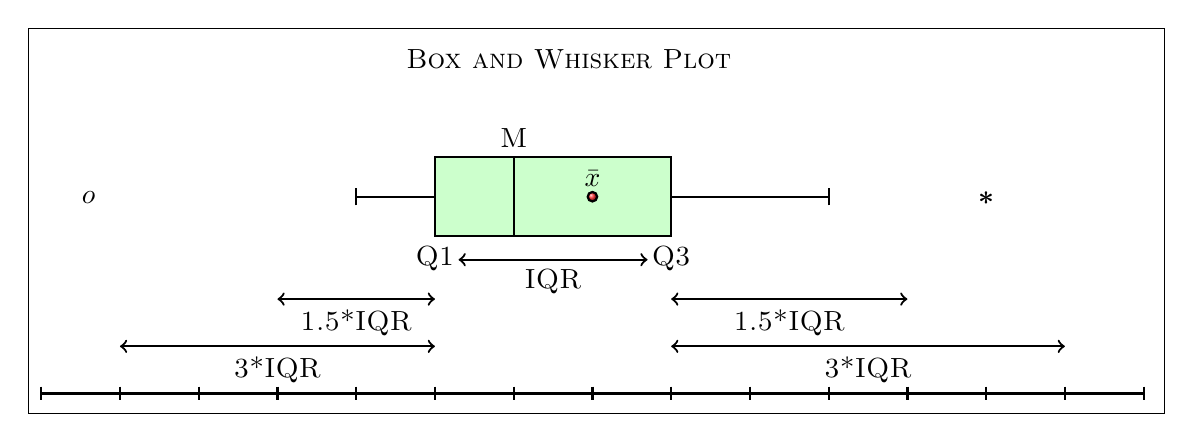
\begin{tikzpicture}[thick, framed]
    \filldraw[fill=green!20] (2,0) rectangle (5,1);% draw the box
    \draw (3,0) -- (3,1) node[above]{$\textsc{M}$};% draw the median
    \draw (5,0.5) -- (7,0.5);% draw right whisker
    \draw (2,0.5) -- (1,0.5);% draw left whisker
    \draw (7,0.39) -- (7,0.61);% draw vertical tab
    \draw (1,0.39) -- (1,0.61);% draw vertical tab
    \node[below] at (2,0) {$\textsc{Q1}$};% label the hinge
    \node[below] at (5,0) {$\textsc{Q3}$};% label the hinge
    \filldraw[ball color=red!80,shading=ball] (4,0.5) circle
        (0.06cm) node[above]{$\bar{x}$};% the mean
    \draw[<->] (2.3, -0.3) -- (4.7, -0.3)
        node[pos=0.5,below]{$\textsc{IQR}$}; % mark the IQR fences
    \draw[<->] (2, -0.8) -- (0,-0.8)
        node[pos=0.5,below]{$\textsc{1.5*IQR}$}; % left inner fence
    \draw[<->] (2,-1.4) -- (-2, -1.4)
        node[pos=0.5,below]{$\textsc{3*IQR}$};% left outer fence
    \draw[<->] (5, -0.8) -- (8,-0.8)
        node[midway,below]{$\textsc{1.5*IQR}$}; % right inner fence
    \draw[<->] (5,-1.4) -- (10, -1.4)
        node[pos=0.5,below]{$\textsc{3*IQR}$};% right outer fence
    %
    \node[below] at (9,0.7) {$\textbf{*}$}; % mild outlier on the right
    \node[below] at (-2.4,0.7) {$o$}; % extreme outlier on the left
    % Title
    \draw (3,2) node[above,xshift=0.7cm]{$ \textsc{Box and Whisker
        Plot}$};%
    % Axis
    \draw (-3,-2) -- (11,-2);
    % Note that the snaked line is drawn to 11.1 to force
    % TikZ to draw the final tick.
    \draw[snake=ticks,segment length=1cm] (-3,-2) -- (11.1,-2);
\end{tikzpicture}

\end{document} 